\subsection{Benutzeroberfläche} \label{subsec:benutzeroberflaeche}

\begin{figure}[H]
		\centering
		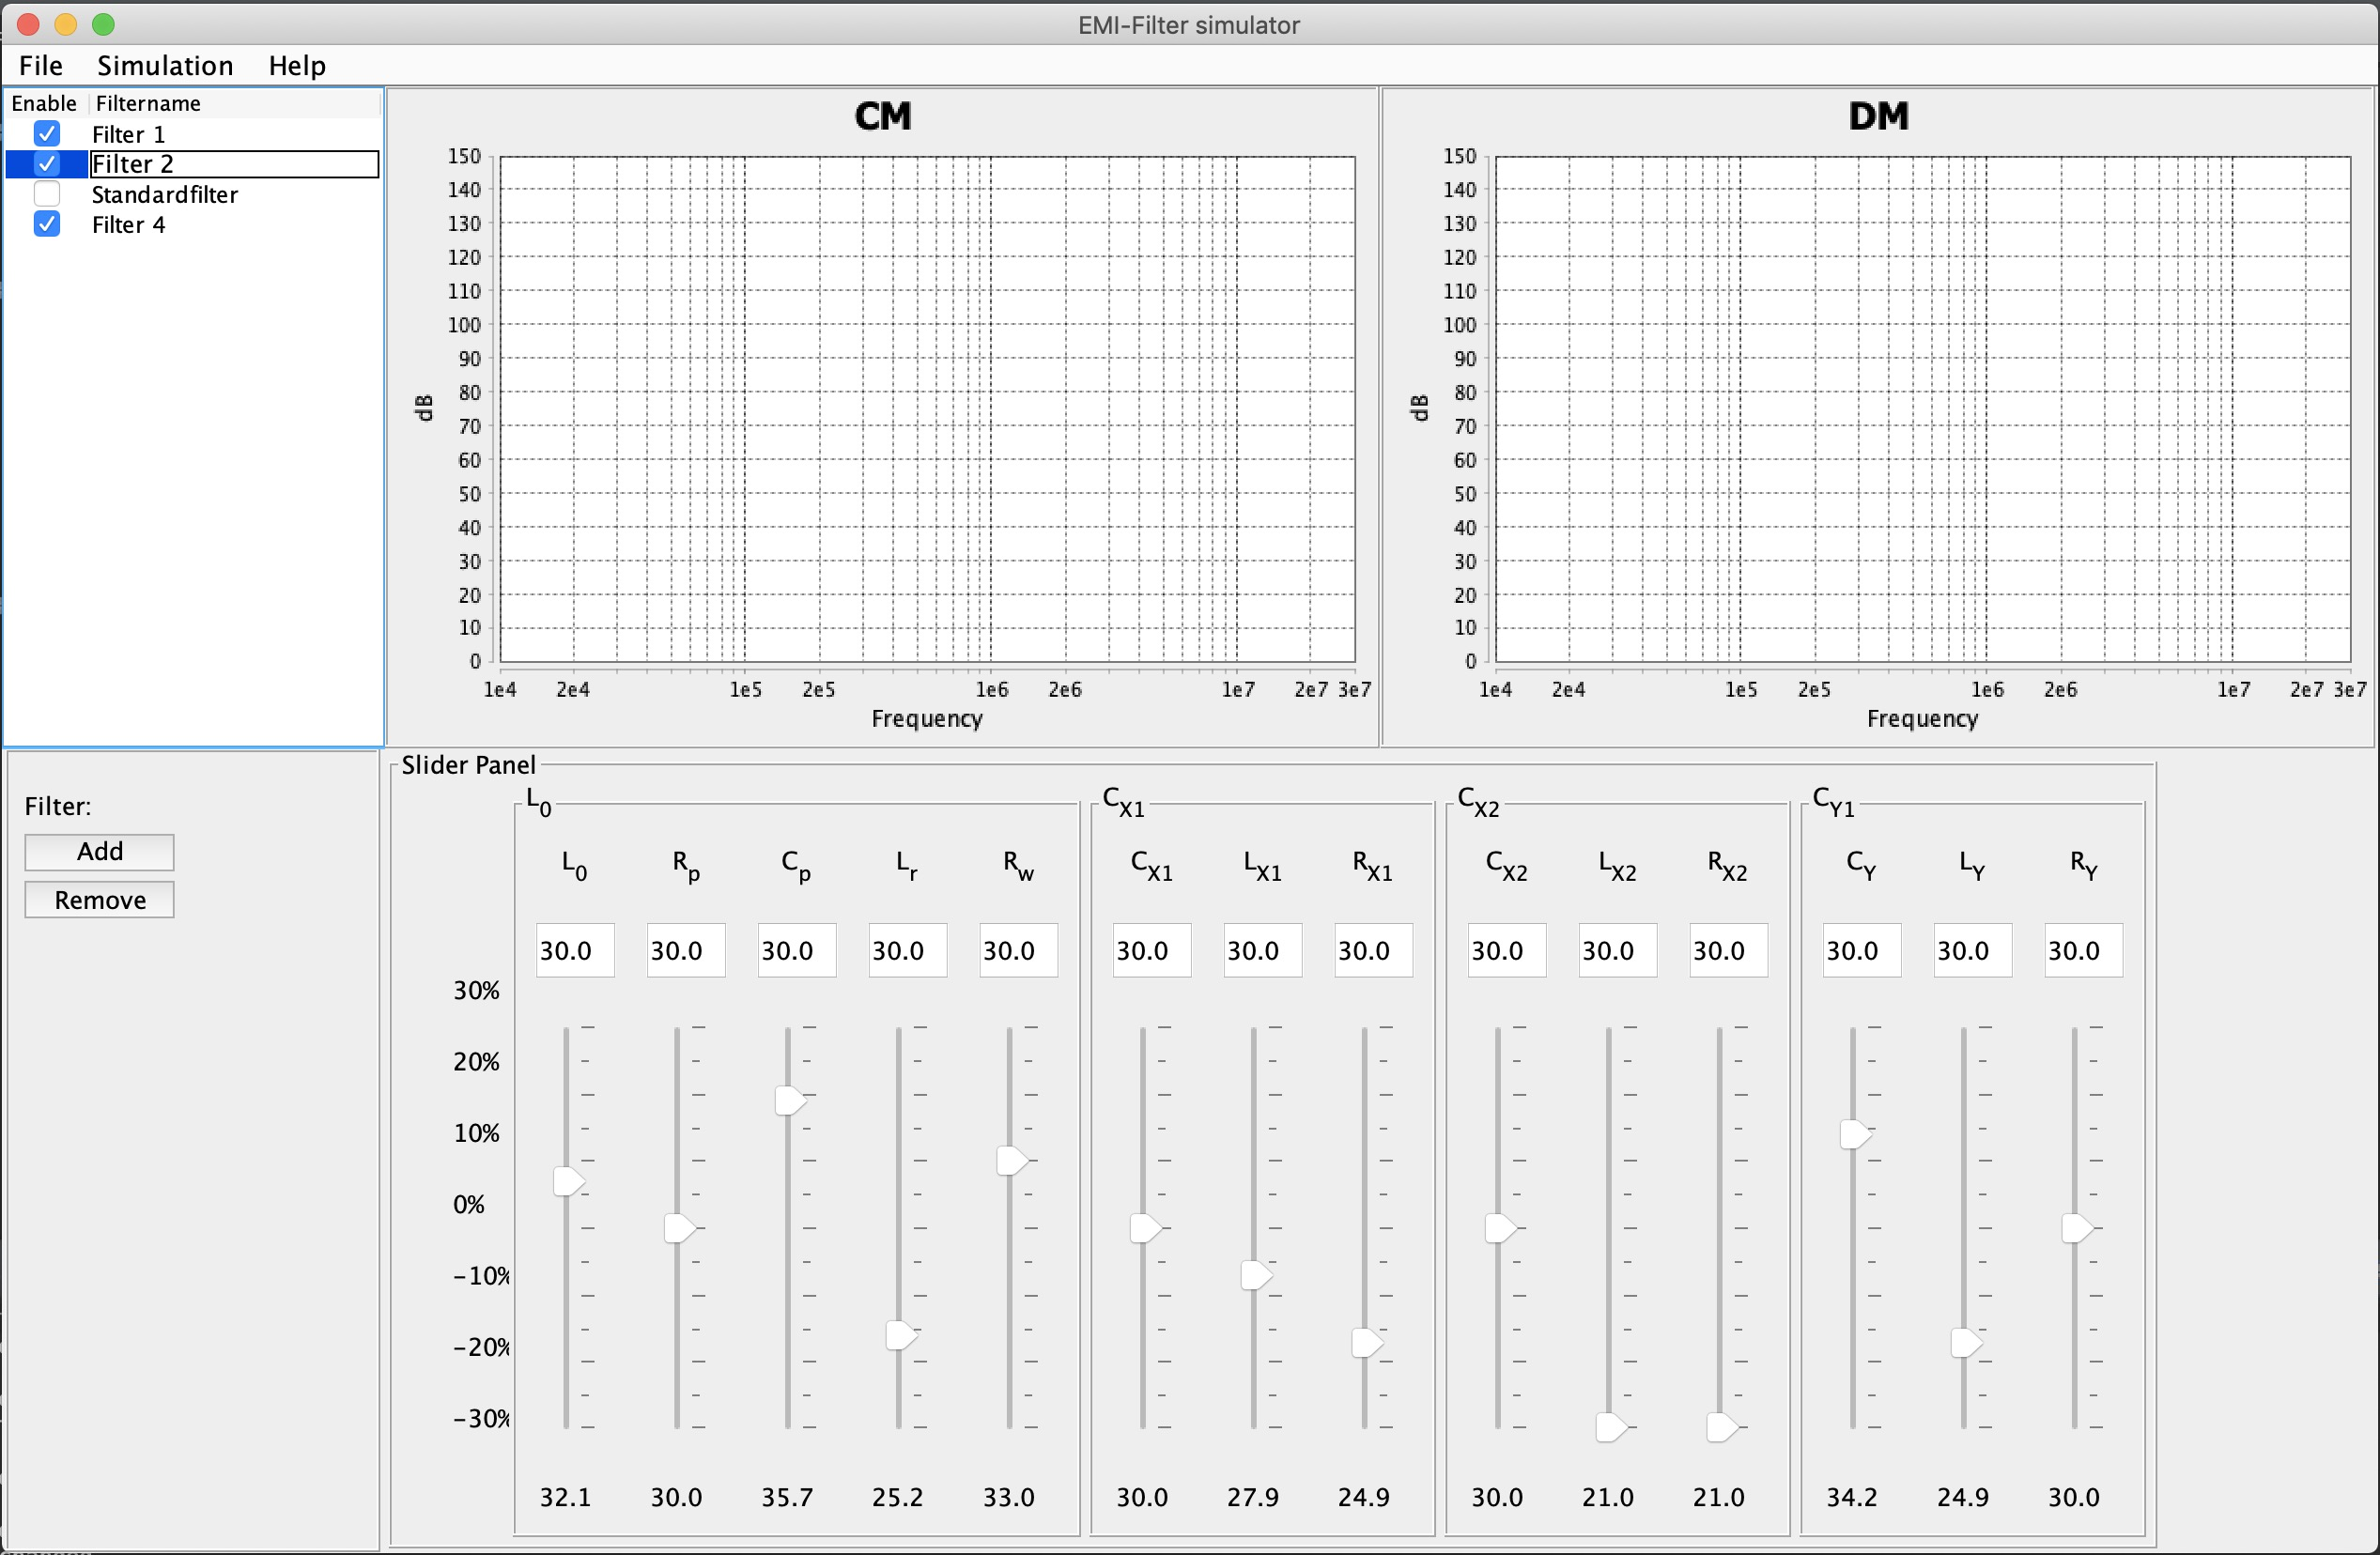
\includegraphics[width = 15cm]{GUI_unfertig.jpg}
		\label{fig:gui}
		\caption{Benutzeroberflächre unfertig}
\end{figure}

Die Oben abgebildete Benutzerfläche ist die Maske, welche sich beim aufstauten der Software auf dem Bildschirm präsentiert.
Wie die  meisten gängigen Applikationen verfügt die GUI eine am oberen Rand platzierten Menubar, um Dateien zu verwalten sowie Hilfestellung zu bieten.
Im Zentrum ist im oberen Bereich das Plotpanel platziert, welches die Simulation sowohl im Gleichtakt (CM), als auch im Gegentakt (DM) als grafische Kurve darstellt.
Gleich unterhalb befindet sich das Inputpanal, es ermöglicht mittels den Textfeldern eine  effiziente Eingabe der Parameter. Mittels den Sleidern können die Parameter prozentual angepasst werden.
Die Filtertabelle links dient zur Verwaltung der Filterprofilen.


\subsubsection{Menu}\label{subsubsec:menu}

Die Menübar verfügt über drei Menüs das File-,  Simulation- und ein Help-Menü.

Das File-Menü dient zur Datenverwaltung, es erlaubt Filterprofile mittels "Save" abzuspeichern und "Load" zu laden. Zudem kann das Programm mittels "Exit" beendet  werden.
Das Programm wandelt das Filterprofiel in ein Komma-getrenntes Textfile.

Mittels "Save" wird das angewählte Filterprofil abgelegt. Es öffnet sich ein Dialog-Fenster,ein File Chooser, dieser erlaubt es den gewünschten Speicherpfad auszuwählen und die Datei zu benennen. Die Eingabe wird mit "Save" bestätigt. Nun ladet das Programm die zugehörigen Arrays, welcher das Filterprofil enthält, mithilfe des Printwriter Koma-getrennt in ein Textfile. Das Textfile wird nun unter dem gewünschten Pfad abgelegt.

Mithilfe von "Load" können





\subsubsection{Plotpanel} \label{subsubsec:plotpanel}


\subsubsection{Inputpanel} \label{subsubsec:inputpanel}



\subsubsection{Filtertabelle} \label{subsubsec:filtertabelle}

